\documentclass[letterpaper]{article} % DO NOT CHANGE THIS
\usepackage[submission]{aaai2027}  % DO NOT CHANGE THIS
\usepackage[hyphens]{url}  % DO NOT CHANGE THIS
\usepackage{graphicx} % DO NOT CHANGE THIS
\urlstyle{rm} % DO NOT CHANGE THIS
\def\UrlFont{\rm}  % DO NOT CHANGE THIS
\usepackage{natbib}  % DO NOT CHANGE THIS AND DO NOT ADD ANY OPTIONS TO IT
\usepackage{caption} % DO NOT CHANGE THIS AND DO NOT ADD ANY OPTIONS TO IT
\frenchspacing  % DO NOT CHANGE THIS
\setlength{\pdfpagewidth}{8.5in} % DO NOT CHANGE THIS
\setlength{\pdfpageheight}{11in} % DO NOT CHANGE THIS
\usepackage{amsmath,amssymb,amsthm}
\usepackage{booktabs}
\usepackage{xcolor}
\pdfinfo{
/TemplateVersion (2027.1)
}
\setcounter{secnumdepth}{0}

\newtheorem{proposition}{Proposition}
\newcommand{\Ltriv}{L_{\mathrm{triv}}}
\newcommand{\kstar}{k^\star}
% Numbers still waiting on runs are marked in red. Remove before submission.
\newcommand{\NEW}[1]{\textcolor{red}{#1}}

\title{Hemodynamic Attenuation: Pruning Attention Heads the Way the Brain Prunes Vessels}
\author{Anonymous Submission}
\affiliations{}

\begin{document}
\maketitle

\begin{abstract}
The brain keeps a blood vessel only while the flow it carries is worth its metabolic upkeep. Vessels that neighbours can cover regress gradually, and new ones sprout where demand returns. We turn this principle into a rule that sizes a transformer's attention during training. Each head gets a valve, and its value is the loss that would remain if it closed and the other heads re-fit to cover for it, the analogue of collateral flow. A head closes, gradually, when its value falls below a fixed upkeep cost. No target size is set. The rule is greedy minimisation of loss plus upkeep, and this makes testable predictions. On a retrieval task whose minimal number of heads $\kstar$ is known, the rule kept exactly $\kstar$ heads in 29 of 30 runs and never broke the model. Three published pruning methods each broke it in every run. The number kept did not depend on the cost until the cost crossed the value of one needed head, where theory predicts a collapse to one head. The collapse occurred there in 36 of 36 runs. On two-layer induction the rule recovered the known previous-token and induction heads in 10 of 10 runs. Under random head failure it kept the number of backup heads predicted before the runs. When the task's demand rose and fell during training, adding sprouting, the analogue of angiogenesis, let the rule regrow the missing heads in 10 of 10 runs and close them again when demand fell.
\end{abstract}

\section{Introduction}

A trained transformer usually has more attention heads than its task needs \citep{michel2019sixteen,voita2019analyzing}, and trained models keep backup heads that take over when others are removed \citep{wang2023interpretability,mcgrath2023hydra}. Existing pruning methods fix the final size by hand, as a target sparsity \citep{zhu2017prune}, a penalty strength \citep{voita2019analyzing} or a threshold \citep{conmy2023towards}, and most prune after training, in one step.

The cerebral circulation solves a similar allocation problem without a target size. Astrocytes and the cells of the neurovascular unit sense local demand and adjust vessel diameter \citep{iadecola2017nvu}. Vessels that carry little flow regress gradually rather than being cut \citep{korn2015pruning}, and tissue survives the loss of a vessel when collateral vessels supply its territory. \citet{murray1926} showed that vessel size follows from minimising the work of moving blood plus the metabolic cost of keeping it. A vessel is kept only while it earns its upkeep. Developing neural circuits likewise overproduce and then prune connections \citep{navlakha2015pruning}.

We carry this principle over to attention heads and call the result \emph{hemodynamic attenuation}. Our contributions are:
\begin{itemize}
\item A rule that values each head by the loss that remains after the other heads compensate for it, charges a fixed upkeep per open head, and closes heads gradually during training, with reopening. It is greedy minimisation of loss plus upkeep (Proposition~1).
\item A benchmark whose minimal circuit is known in size and roles, and a prediction of the cost range in which the rule recovers it, confirmed in 36 of 36 runs.
\item Evidence that the rule recovers the minimal count without breaking the model, recovers the induction circuit, keeps a predicted number of backups under damage, and, with sprouting, regrows heads when demand returns and closes them when it falls.
\end{itemize}

\section{Hemodynamic Attenuation}

\paragraph{Valves.} Each head's output passes through a valve $g_h\in[0,1]$ before the heads are summed, $\hat{T}=\sum_h g_h\, O_h W_O^h$. A head with $g_h=0$ adds nothing and receives no gradient, so a model with $k$ open valves is exactly a $k$-head model.

\paragraph{Collateral value.} For the set $S$ of open heads, let $L^\ast(S)=\min_{W_O} L$ be the loss after the output weights of the heads in $S$ are re-fitted, with their attention held fixed. The collateral value of an open head is $v_h=L^\ast(S\setminus h)-L^\ast(S)$, and the gain of a closed head is $L^\ast(S)-L^\ast(S\cup h)$. Both come in closed form from one inverse of the heads' output covariance on a batch of cached outputs. The score is the Optimal Brain Surgeon score \citep{obs} applied to whole heads, as in ZipLM \citep{ziplm}. What is new is its use. The re-fit is the analogue of collateral flow and makes a copy worthless. If two heads output the same signal, the survivor takes over its twin's weight and the loss does not change.

\paragraph{Schedule.} All valves start open. After a warm-up of 10\% of training, every 25 steps the rule (1) computes all values, (2) closes the lowest-valued open head if $v_h<\pi$, and otherwise (3) reopens the highest-gain closed head if its gain exceeds $2\pi$. A closing valve falls by $1/100$ per step, so a head regresses over 100 steps while the others adapt. The upkeep is $\pi=0.03\,\Ltriv$, where $\Ltriv$ is the loss of predicting the mean.

\paragraph{The rule optimises an objective.} Let $J(S)=L^\ast(S)+\pi|S|$, the loss plus the upkeep of the open heads, which is the form of Murray's cost.
\begin{proposition}
Closing $h$ lowers $J$ exactly when $v_h<\pi$, and reopening $h$ lowers $J$ by more than $\pi$. At a fixed point of the rule, no single removal lowers $J$, and no single addition lowers it by more than $\pi$. If needed heads are worth more than $\pi$ and redundant heads less, the fixed point keeps the needed heads and only those, for any such $\pi$.
\end{proposition}
The first two claims follow from $J(S\setminus h)-J(S)=v_h-\pi$ and $J(S\cup h)-J(S)=\pi-\mathrm{gain}_h$. The rule is therefore forward--backward greedy selection \citep{zhang2011foba} over groups of weights, run while the heads themselves are still learning. The fade and the warm-up handle the fact that $L^\ast$ changes as the heads train. The proposition makes a falsifiable prediction. The number of heads kept should not depend on $\pi$ while $\pi$ lies between the value of a redundant head and the value of a needed one, and it should change abruptly when $\pi$ leaves that range.

\section{A Benchmark with a Known Minimal Circuit}

A memory of $N=16$ slots holds random items $c_j$, redrawn for every example. A query names a position $p$, and the target is the $R$ items at fixed offsets, $(c_{p+\delta_1},\dots,c_{p+\delta_R})$, slots taken modulo $N$. A head returns one weighted average of the items per query, which is one linear combination of the $R$ unknowns, so recovering $R$ items needs $R$ heads with different attention patterns, one per offset. With $k\le R$ such heads the lowest achievable loss is
\begin{equation}
L^\ast(k)=\left(1-k/R\right)\Ltriv ,
\label{eq:law}
\end{equation}
which we confirmed on trained models to within $0.003\,\Ltriv$. A copy of a head adds nothing. Each needed head is therefore worth $\Ltriv/R$ and each redundant head $0$, so Proposition~1 predicts exactly $\kstar=R$ heads for any $\pi<\Ltriv/R$, and a collapse to a single head for $\pi>\Ltriv/R$, where every needed head costs more than it saves. The model is one cross-attention layer with $H=32$ heads, width 128, head width 32 and no MLP. The task is solved when the loss is below $0.02\,\Ltriv$ ($R^2\ge0.98$). We report \emph{exact count} (open heads over the last 40\% of training equal $\kstar$) and \emph{never broke} (once solved, the loss never rises above the bar).

\begin{figure*}[t]
\centering
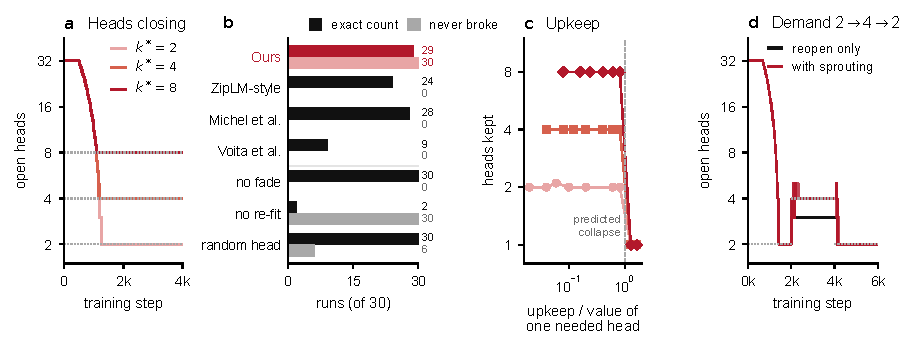
\includegraphics[width=\textwidth]{fig_neuroai.pdf}
\caption{\textbf{(a)} Open heads during training, one run per task size, with $\kstar$ dotted. \textbf{(b)} Every method on the same 30 runs ($\kstar=2,4,8$, 10 seeds each): runs with exactly $\kstar$ heads (dark) and runs that never broke (light). \textbf{(c)} Heads kept against the upkeep $\pi$, in units of the value of one needed head, $\Ltriv/R$. Theory predicts $\kstar$ heads to the left of 1 and one head to the right. \textbf{(d)} Demand rises from 2 to 4 offsets and falls back to 2 during training, 10 runs each. Reopening alone (black) stalls at 3 heads in 8 of 10 runs; with sprouting (red) every run regrows to 4 and returns to 2.}
\label{fig:results}
\end{figure*}

\section{Results}

\paragraph{Exact count without breaking the model.} The rule kept exactly $\kstar$ heads in 29 of 30 runs and never broke the model in 30 of 30 (Figure~\ref{fig:results}a,b). We implemented three published methods in the same training runs. Michel et al.\ \citep{michel2019sixteen}, given the true count, kept it in 28 of 30 runs. ZipLM-style pruning \citep{ziplm}, which applies the same score once and then fine-tunes, kept it in 24 of 30. Learned $L_0$ gates \citep{voita2019analyzing,louizos2018learning} kept it in 9 of 30. All three broke the model in every run. Removing one part of the rule at a time shows what each part does. Without the fade the model broke in every run, like vessels cut rather than regressed. Without the re-fit, which is the Optimal Brain Damage score \citep{obd}, the rule kept too many heads (2 of 30 exact) because it valued copies. With a random choice of head it broke the model in 24 of 30 runs. When every head started with an exact twin, the rule kept 4 heads and never both members of a pair in 10 of 10 runs, while the score without re-fit kept 8 to 15 heads.

\paragraph{The cost does not set the size, until theory says it should.} Every upkeep from $0.01$ to $0.1\,\Ltriv$ gave the exact count at $\kstar=2,4,8$. Proposition~1 predicts where this stops. Above $\pi=\Ltriv/R$ every needed head costs more than it saves, so the rule should close heads down to one. We set $\pi$ at 0.6, 0.8, 1.25 and 1.6 times $\Ltriv/R$ for $\kstar=2,4,8$, with 3 seeds each. All 18 runs below the breakpoint kept exactly $\kstar$ heads, and all 18 above it kept one (Figure~\ref{fig:results}c). The final loss of the collapsed runs was $0.50$, $0.75$ and $0.875\,\Ltriv$, which is Equation~\eqref{eq:law} with $k=1$. The size is set by the task, and the range of costs that recover it is known in advance.

\paragraph{Backup heads under damage.} If each head fails with probability $p$ at every step, a head is worth keeping only when it is likely to be needed. Averaging the collateral value over failure patterns gives the expected value of the $B$-th head, $v(B)=\frac{1-p}{R}\Pr[\mathrm{Bin}(B-1,1-p)<R]\,\Ltriv$, and the predicted count is the largest $B$ with $v(B)\ge\pi$. We wrote these predictions down before the runs. They matched in 25 of 30 runs, and the rest were off by one head. Like collaterals, which develop where occlusion is likely, backup heads appear only when failure makes them worth their upkeep.

\paragraph{A second circuit: induction.} A two-layer attention-only model with $8+8$ heads was trained to continue a repeated sequence of tokens. Its known minimal circuit is a previous-token head in layer 1 and an induction head in layer 2 \citep{olsson2022}. Cross-entropy has no closed-form re-fit, so here a head is valued by the loss without it. The rule kept $2+1$ heads in 10 of 10 runs and never broke the model, and reopening fired 2 to 7 times per run. The kept heads had the expected roles in every run. Switching off the layer-2 head reduced next-token accuracy on the repeat from 99.9\% to 1.8\%, chance for 64 tokens. Layer 1 kept two heads that each missed about 1 in 8 repeated tokens alone and about 1 in 200 together. Michel et al.\ broke the model in all 10 runs.

\paragraph{Changing demand.} Vascular networks also grow where demand returns. We tested this by changing the task during training. The run is split into three equal phases of 2{,}000 steps, in which 2, then 4, then 2 of the four offsets are active, the targets of the inactive offsets being zero. A model with two heads cannot solve the middle phase, since by Equation~\eqref{eq:law} its loss cannot fall below $0.5\,\Ltriv$. With reopening alone, only 2 of 10 runs recovered. In the other 8 the rule reopened one head, which learned one new offset, and then stalled at 3 heads with a loss of $0.25\,\Ltriv$ for the whole phase (Figure~\ref{fig:results}d). The reason is that a closed head receives no gradient, so it cannot learn the new offset, and its gain stays below $2\pi$. We therefore added \emph{sprouting}, the analogue of angiogenesis driven by hypoxic tissue. If the loss stays above the solved bar for four consecutive checks, the closed head with the highest gain is opened even below $2\pi$, so that it can learn, and the rule closes it again if it does not earn its upkeep. With sprouting, 10 of 10 runs reached exactly 4 heads and solved the task within 100 to 300 steps of the change. When demand fell, all 20 runs closed back to exactly 2 heads within 180 steps.

\paragraph{Size.} With exactly $\kstar$ heads, deleting the closed heads leaves 6.3\% to 25\% of the retrieval model's parameters (12.5\% for $\kstar=4$), and 30.3\% of the induction model's. Counting only open heads, training used 0.31 to 0.45 of the dense model's head-steps.

\section{Discussion}

The vascular principle that a vessel stays only while it earns its upkeep gives a pruning rule with no target size. It also gives an objective, and the objective predicts where the rule works and where it fails. Three properties come from the biology, and each is needed. The re-fit plays the role of collateral flow and removes copies. Gradual regression keeps the model intact. Reopening and sprouting play the role of regrowth, and sprouting is needed because a closed head, like a regressed vessel, cannot adapt until it is supplied again. The correspondence is a design principle, not a model of cerebral blood flow.

\paragraph{Limitations.} The tasks are small and synthetic, chosen so that the minimal circuit is known, and the retrieval model has a single layer. The re-fit is exact only for the output weights. On induction the rule kept one layer-1 head more than the minimum, and a value that re-fits each layer to rebuild what the next layer reads may close it. Closed heads are still computed during training, so the saving in training compute is nominal until they are deleted. Next we will apply the rule to a cross-attention model of two wearable signals, chest and wrist, and to GPT-2 small on indirect object identification, whose circuit is known \citep{wang2023interpretability}.

\bibliography{refs}

\end{document}
